% !TeX spellcheck = en_US
% !TeX encoding = utf8
% !TeX program = xelatex
% !BIB program = bibtex

\documentclass[notes]{beamer}
% \documentclass[draft]{beamer}	
\usetheme{Singapore}
% \usetheme{Hannover}
%\usepackage{pgfpages}
%\setbeameroption{show notes on second screen}

\usepackage[british]{babel}
\usepackage{graphicx,hyperref,url}
% \usepackage{ru}
\usepackage{mmstyles}
% \usepackage{hanging}
\usepackage{listings}
\usefonttheme[onlymath]{serif}
\usepackage{fontspec}
\usepackage{xeCJK}
% \pgfdeclareimage[width=\paperwidth,height=\paperheight]{bg}{background}
% \setbeamertemplate{background}{\pgfuseimage{bg}}

% \usepackage[backend=biber]{biblatex}
% \bibliography{./ref.bib}
%\addbibresource{ref.bib}
\usepackage{indentfirst}
\usepackage{longtable}
\usepackage{float}
%\usepackage{picins}
\usepackage{rotating}
\usepackage{subfigure}
\usepackage{tabu}
\usepackage{amsmath}
\usepackage{amssymb}
\usepackage{setspace}
\usepackage{amsfonts}
\usepackage{appendix}
\usepackage{listings}
\usepackage{xcolor}
\usepackage{geometry}
% \setCJKfamilyfont{cjkhwxk}{SimSun}
% \newcommand*{\cjkhwxk}{\CJKfamily{cjkhwxk}}
%\newfontfamily{\consolas}{Consolas}
%\newfontfamily{\monaco}{Monaco}
%\setmonofont[Mapping={}]{Consolas}	%英文引号之类的正常显示,相当于设置英文字体
%\setsansfont{Consolas} %设置英文字体 Monaco, Consolas,  Fantasque Sans Mono
% \setmainfont{Times New Roman}
% \newfontfamily{\consolas}{Times New Roman}
% \newfontfamily{\monaco}{Arial}
% \setCJKmainfont{Times New Roman}
%\setmainfont{MONACO.TTF}
%\setsansfont{MONACO.TTF}
\newcommand{\verylarge}{\fontsize{60pt}{\baselineskip}\selectfont}  
\newcommand{\chuhao}{\fontsize{44.9pt}{\baselineskip}\selectfont}  
\newcommand{\xiaochu}{\fontsize{38.5pt}{\baselineskip}\selectfont}  
\newcommand{\yihao}{\fontsize{27.8pt}{\baselineskip}\selectfont}  
\newcommand{\xiaoyi}{\fontsize{25.7pt}{\baselineskip}\selectfont}  
\newcommand{\erhao}{\fontsize{23.5pt}{\baselineskip}\selectfont}  
\newcommand{\xiaoerhao}{\fontsize{19.3pt}{\baselineskip}\selectfont} 
\newcommand{\sihao}{\fontsize{14pt}{\baselineskip}\selectfont}      % 字号设置  
\newcommand{\xiaosihao}{\fontsize{12pt}{\baselineskip}\selectfont}  % 字号设置  
\newcommand{\wuhao}{\fontsize{10.5pt}{\baselineskip}\selectfont}    % 字号设置  
\newcommand{\xiaowuhao}{\fontsize{9pt}{\baselineskip}\selectfont}   % 字号设置  
\newcommand{\liuhao}{\fontsize{7.875pt}{\baselineskip}\selectfont}  % 字号设置  
\newcommand{\qihao}{\fontsize{5.25pt}{\baselineskip}\selectfont}    % 字号设置 

\graphicspath{{./fig/}}

% \setbeamertemplate{footnote}{%
%   \hangpara{2em}{1}%
%   \makebox[2em][l]{\insertfootnotemark}\footnotesize\insertfootnotetext\par%
% }

\definecolor{cred}{rgb}{0.6,0,0}
\definecolor{cgreen}{rgb}{0.25,0.5,0.35}
\definecolor{cpurple}{rgb}{0.5,0,0.35}
\definecolor{cdocblue}{rgb}{0.25,0.35,0.75}
\definecolor{cdark}{rgb}{0.95,1.0,1.0}
\lstset{
	language=R,
	numbers=left,
	numberstyle=\tiny\color{black},
	keywordstyle=\color{cpurple}\consolas,
	commentstyle=\color{cgreen}\consolas,
	stringstyle=\color{cred}\consolas,
	frame=single,
	escapeinside=``,
	xleftmargin=1em,
	xrightmargin=1em, 
	backgroundcolor=\color{cdark},
	aboveskip=1em,
	breaklines=true,
	tabsize=3
} 

\providecommand{\tightlist}{%
  \setlength{\itemsep}{0pt}\setlength{\parskip}{0pt}}

  
% The title of the presentation:
%  - first a short version which is visible at the bottom of each slide;
%  - second the full title shown on the title slide;
\title[Opt for ML]{Perceptons}

% Optional: a subtitle to be dispalyed on the title slide
% \subtitle{Optimization for Machine Learning}

% The author(s) of the presentation:
%  - again first a short version to be displayed at the bottom;
%  - next the full list of authors, which may include contact information;
\author[YingmingLi]{Yingming Li \\ yingming@zju.edu.cn}
% The institute:
%  - to start the name of the university as displayed on the top of each slide
%    this can be adjusted such that you can also create a Dutch version
%  - next the institute information as displayed on the title slide

\institute[DSERC, ZJU]{Data Science \& Engineering Research Center, ZJU}

% Add a date and possibly the name of the event to the slides
%  - again first a short version to be shown at the bottom of each slide
%  - second the full date and event name for the title slide
\date[\today]{\today}

\begin{document}

\AtBeginSection[]
{
	\begin{frame}
		\frametitle{Outline}
		\tableofcontents[currentsection]
	\end{frame}
}

% \AtBeginSubsection[2-]
% {
%    \begin{frame}
%        \frametitle{Outline}
%        \tableofcontents[currentsection]
%    \end{frame}
% }


\begin{frame}
	\titlepage
	\begin{center}
		Adapted from slides provided by Prof. Jihun Hamm.		
	\end{center}

\end{frame}

\section{Definition}\label{definition}

\subsection{}\label{section}

\begin{frame}{Perceptrons}

\begin{itemize}
\tightlist
\item
  Architecture: one-layer feedforward net

  \begin{itemize}
  \tightlist
  \item
    Without loss of generality, consider a single-neuron perceptron
  \end{itemize}
\end{itemize}

\centering
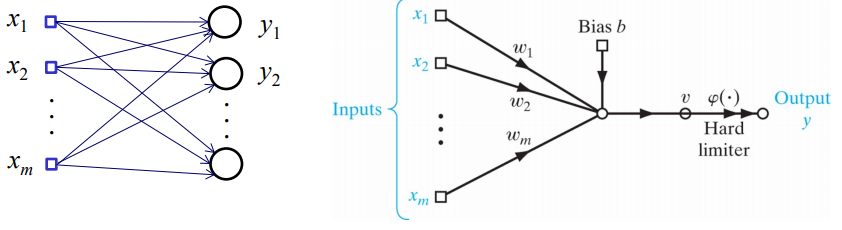
\includegraphics[width=0.85000\textwidth]{2018-03-08-21-55-42.png}\\

\end{frame}

\begin{frame}{Definition}

\[y=\varphi(\nu)\] \[\nu=\sum_{i=1}^{m} w_i x_i +b \]

\[\varphi (\nu) = \left\{ \begin{array}{cc}
    1  & \text{ if } \nu \ge 0 \\ 
    -1 & \text{ otherwise } 
    \end{array} \right. \]

Hence a McCulloch-Pitts neuron, but with real-valued inputs

\end{frame}

\begin{frame}{Pattern recognition}

\begin{itemize}
\tightlist
\item
  With a bipolar output, the perceptron performs a 2-class
  classification problem, \ie, apples vs.~oranges.
\item
  How do we learn to perform classification?
\item
  The perceptron is given pairs of input \(x_p\) and desired output
  \(d_p\)
\item
  How can we find \(y_p = \varphi (x_p^T w) =d_p, \forall p\)
\end{itemize}

\end{frame}

\subsection{Decision boundary}\label{decision-boundary}

\begin{frame}{But first: decision boundary}

\begin{itemize}
\tightlist
\item
  Can we visualize the decision the perceptron would make in classifying
  every potential point?
\item
  Yes, it is called the discriminant function
  \[g(x)=x^Tw=\sum_{i=0}^{m} w_i x_i\]
\item
  What is the boundary between the two classes like?
\item
  This is a linear function of x
\end{itemize}

\end{frame}

\begin{frame}{Decision boundary example}

\centering 

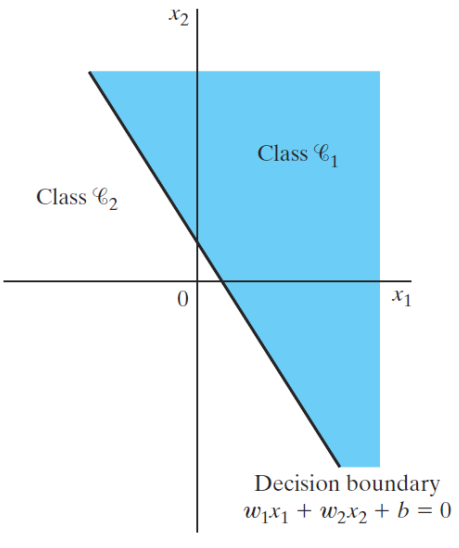
\includegraphics[width=0.50000\textwidth]{2018-03-08-22-28-01.png}\\

\end{frame}

\begin{frame}{Decision boundary}

\begin{itemize}
\tightlist
\item
  For an m-dimensional input space, the decision boundary is an
  \((m-1)\)-dimensional hyperplane perpendicular to \(w\). The
  hyperplane separate the input space into two halves, with one half
  having \(y=1\), and the other half having \(y=-1\)

  \begin{itemize}
  \tightlist
  \item
    When \(b=0\), the hyperplane goes through the origin.
  \end{itemize}
\end{itemize}

\centering 

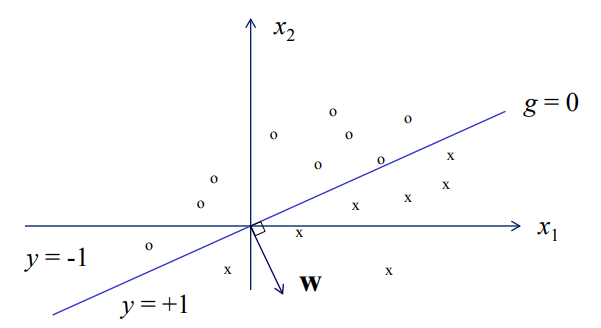
\includegraphics[width=0.70000\textwidth]{2018-03-08-22-30-37.png} ~

\end{frame}

\begin{frame}{Linear separability}

\begin{itemize}
\tightlist
\item
  For a set of input patterns \(x_p\), if there exists at least one
  \(w\) that separates \(d=1\) patterns from \(d=-1\) patterns, then the
  classification problem is linearly separable.

  \begin{itemize}
  \tightlist
  \item
    In other words, there exists a linear discriminant function that
    produces no classification error.
  \item
    Examples: AND, OR, XOR
  \end{itemize}
\end{itemize}

\end{frame}

\begin{frame}{Linear separability}

\begin{figure}
\centering
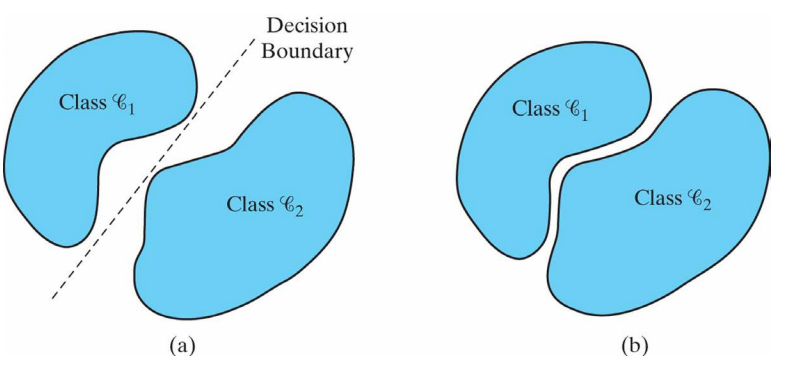
\includegraphics[width=0.90000\textwidth]{2018-03-08-22-36-07.png}
\caption{illustration: \textbf{left}: Linear separable, \textbf{right}:
Not linear separable}
\end{figure}

\end{frame}

\begin{frame}{Perceptron definition (recap. )}

\[y=\varphi(\nu)\] \[\nu=\sum_{i=1}^{m} w_i x_i +b \]

\[\varphi (\nu) = \left\{ \begin{array}{cc}
    1  & \text{ if } \nu \ge 0 \\ 
    -1 & \text{ otherwise } 
    \end{array} \right. \]

Hence a McCulloch-Pitts neuron, but with real-valued inputs

\end{frame}

\section{Learning rule}\label{learning-rule}

\subsection{}\label{section-1}

\begin{frame}{Perceptron learning rule}

\begin{itemize}
\tightlist
\item
  Learn parameters \(w\) from examples \((x_p,d_p)\)
\item
  In an online fashion, \ie, one point at a time
\item
  Adjust weights as necessary, \ie, when incorrect
\item
  Adjust weights to be more like \(d=1\) points and more like negative
  \(d=-1\) points.
\end{itemize}

\end{frame}

\begin{frame}{Biological analogy}

\begin{itemize}
\tightlist
\item
  Strengthen an active synapse if the postsynaptic neuron fails to fire
  when it should have fired
\item
  Weaken an active synapse if the neuron fires when it should not have
  fired
\item
  Formulated by Rosenblatt based on biological intuition
\end{itemize}

\end{frame}

\begin{frame}{Quantitatively}

\begin{equation} 
\begin{aligned} 
w(n+1) & = w(n) + \Delta w(n) \\ 
 & = w(n) + \eta [d(n)-y(n)]x(n) \\
\end{aligned}
\end{equation}

\begin{itemize}
\tightlist
\item
  \(n\): iteration number, iterating over points in turn
\item
  \(\eta\): step size or learning rate
\item
  Only updates \(w\) when \(y(n)\) is incorrect
\end{itemize}

\end{frame}

\begin{frame}{Geometric interpretation}

\centering 

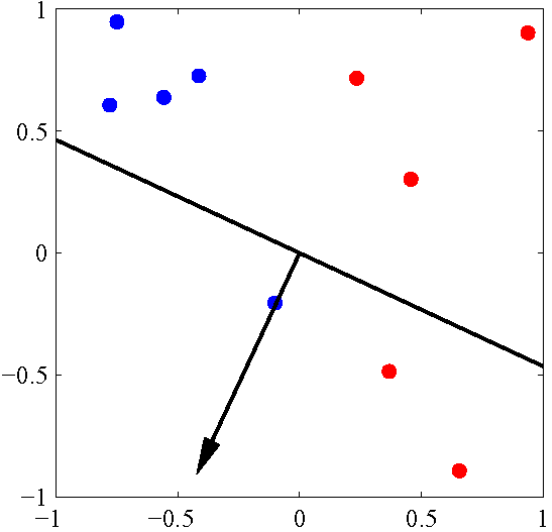
\includegraphics[width=0.55000\textwidth]{2018-03-08-22-45-16.png}\\

\end{frame}

\begin{frame}{Geometric interpretation}

\centering 

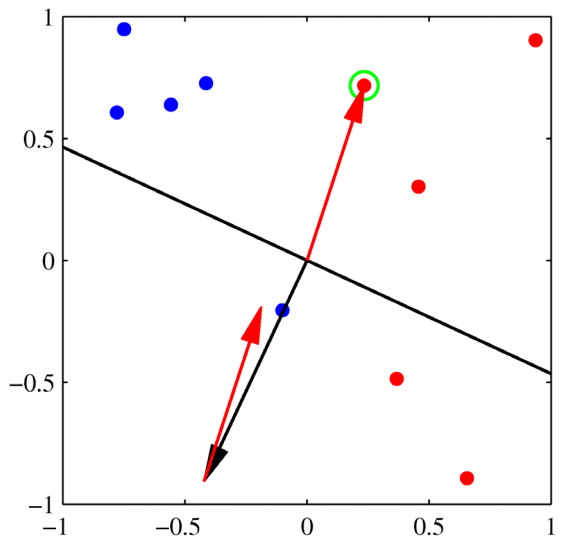
\includegraphics[width=0.55000\textwidth]{2018-03-08-22-45-53.png}\\

\end{frame}

\begin{frame}{Geometric interpretation}

\centering 

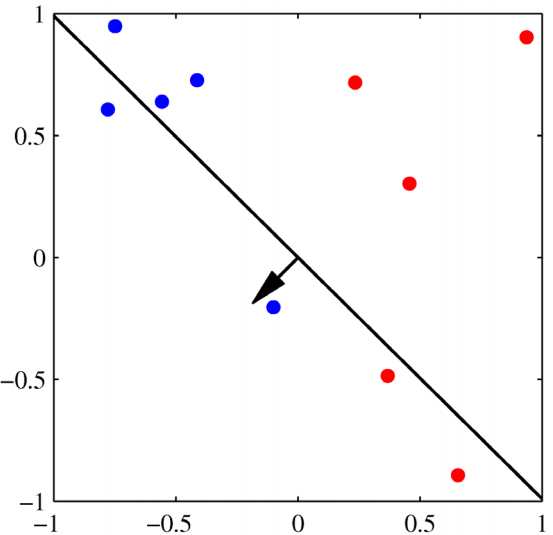
\includegraphics[width=0.55000\textwidth]{2018-03-08-22-46-08.png}\\

\end{frame}

\begin{frame}{Geometric interpretation}

\centering 

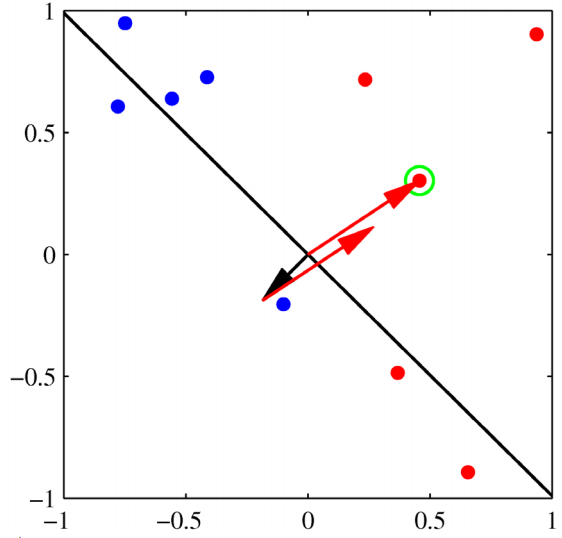
\includegraphics[width=0.55000\textwidth]{2018-03-08-22-46-39.png}\\

\end{frame}

\begin{frame}{Geometric interpretation}

\centering 

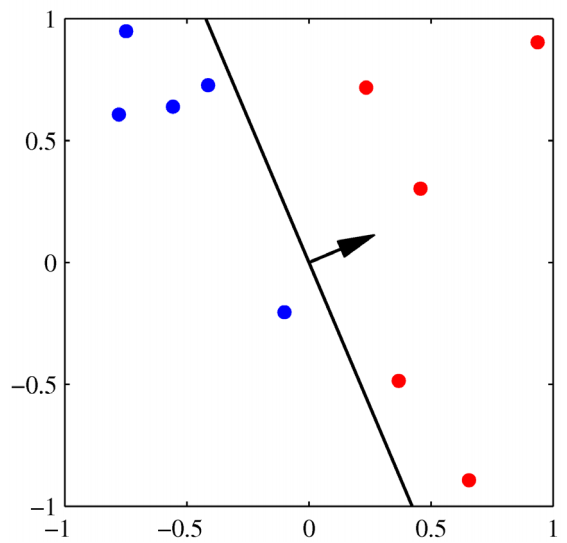
\includegraphics[width=0.55000\textwidth]{2018-03-08-22-48-52.png}\\

\end{frame}

\begin{frame}{Geometric interpretation}

\begin{itemize}
\tightlist
\item
  Each weight update moves \(w\) closer to \(d = 1\) patterns, or away
  from \(d = -1\) patterns.
\item
  Final weight vector in example solves the classification problem
\item
  Is that true in all cases?
\end{itemize}

\end{frame}

\begin{frame}{Summary of perceptron learning algorithm}

\begin{itemize}
\tightlist
\item
  Definition:

  \begin{itemize}
  \tightlist
  \item
    \(w(n)\): (m+1)-by-1 weight vector (including bias) at step n
  \end{itemize}
\item
  Inputs:

  \begin{itemize}
  \tightlist
  \item
    \(x(n)\): \(n^{th}\) (m+1)-by-1 input vector with first element = 1
  \item
    \(d(n)\): \(n^{th}\) desired response
  \end{itemize}
\item
  Initialization: set \(w(0)=0\)
\item
  Repeat until no points are mis-classified

  \begin{itemize}
  \tightlist
  \item
    Compute response: \(y(n)=\mathrm{sgn}\left[w(n)^T x(n) \right]\)
  \item
    Update: \(w(n+1)=w(n) + \left[d(n) -y(n) \right]x(n)\)
  \end{itemize}
\end{itemize}

\end{frame}

\begin{frame}
	\chuhao Thank you! %\fontspec{LHANDW.TTF}
\end{frame}


\end{document}
